\documentclass[journal]{IEEEtran}

\usepackage{cite}
\usepackage[pdftex]{graphicx}
\usepackage[tight,footnotesize]{subfigure}
\usepackage[portuguese]{babel}
\usepackage[utf8]{inputenc}
\usepackage[T1]{fontenc}
\usepackage{geometry}
\usepackage{caption}
\usepackage{float}
\usepackage{tabularx}
\usepackage{multirow}
\usepackage[bookmarks]{hyperref}
\usepackage{hypcap}
\usepackage{amsfonts}
\usepackage{amssymb}

\hyphenation{}

\begin{document}
\title{Sistema Operativo de Tempo Real para ATmega baseado em microkernel preemptivo}
\author{Rui Graça (201004124), Eduardo Almeida (201000641), Tiago Costa (200601289)}

\markboth{Sistemas Embarcados - FEUP 2013/14}%
{}

\IEEEspecialpapernotice{Relatório}

\maketitle


\begin{abstract}
	O produto do trabalho realizado é um sistema operativo de tempo real (RTOS) baseado num microkernel preemptivo, tendo como tecnologia alvo o microcontrolador
	ATmega328P.

	O sistema desenvolvido implementa stacks separadas para cada tarefa e escalonamento baseado em prioridades fixas, sendo que a API oferece funções como temporizadores,
	sinalização para sincronização entre tarefas e semáforos, baseados em SRP, assim como a possibilidade de lançar novas tarefas durante a execução do sistema.
\end{abstract}

\section{Introdução}
\IEEEPARstart{O}{s} requisitos temporais a que estão sujeitos sistemas de tempo real levam à necessidade da utilização de sistemas operativos adequados, que permitam um
comportamento totalmente determinístico, em que pode ser feita, de forma simples, uma análise do cumprimento dos requisitos temporais.

O trabalho aqui apresentado tem como produto final um sistema operativo que se enquadra neste contexto, possibilitando ao programador de sistemas de tempo real garantias
de um comportamento determinístico e uma interface (API) com funcionalidades básicas para a implementação de um sistema de tempo real.

O sistema desenvolvido é um sistema com preempção, o que significa que existe uma interrupção periódica (tick) que verifica qual é a tarefa de maior prioridade pronta a
executar e atribui-lhe o CPU.
Cada tarefa representa uma thread de funcionamento do sistema, à qual é atribuída uma stack independente, que mantém o seu contexto entre as suas diversas ativações.
Para isto, é necessário que, na troca de contexto, o stack pointer seja devidamente alterado.

O lançamento de novas tarefas pode ser feito tanto na inicialização do sistema como durante a execução, permitindo a uma tarefa lançar uma nova tarefa.
Não existe, no entanto, nenhuma relação hierárquica entre tarefas criadoras e criadas, nem nenhuma relação especial entre elas.

Na API do sistema operativo são fornecidas funções que possibilitam a criação de temporizadores periódicos, que podem ser locais às tarefas que os criam ou globais, sendo
que, neste caso, várias tarefas podem esperar por um mesmo temporizador.
Após a criação de um temporizador, uma tarefa pode invocar uma função que espera que seja ativada por esse temporizador, colocando a tarefa num estado inativo e
adicionando a tarefa à lista de espera do temporizador, que é esvaziada no tick do sistema, ativando todas as tarefas nela existentes.

A API possibilita, também, que uma tarefa fique inativa e seja acordada após um tempo determinado.
Esta funcionalidade não é mais que a criação temporária de um temporizador.

Outra funcionalidade de extrema importância em sistemas com preempção são os semáforos, que controlam o acesso a regiões críticas, impedindo que a sequência de execução
de tarefas tenha consequências imprevistas e indesejadas, as chamadas race conditions.
Em sistemas de tempo real, dado que o escalonamento é baseado em prioridades, a utilização de semáforos como implementados noutros sistemas é problemática, dado que causa
inversão de prioridade não limitada, que acontece quando uma tarefa de alta prioridade pode ficar ilimitadamente bloqueada porque necessita que uma tarefa de mais baixa
prioridade liberte um semáforo, sendo que esta tarefa de mais baixa prioridade não poderá executar enquanto houver tarefas de prioridade intermédia a ocupar o CPU.
Surge, desta forma, a necessidade de mecanismos de controlo de race conditions que limitem ao mínimo a inversão de prioridade.
Estes mecanismos passam, em geral, por uma herança temporária de prioridade, em que a tarefa que tem um semáforo (no qual está bloqueada uma tarefa de prioridade
superior) fica temporáriamente com uma prioridade superior à original.

O mecanismo utilizado no sistema apresentado baseia-se em Stack Resource Policy (SRP), implementando semáforos binários (mutexes).
De acordo com este protocolo, existe um teto do sistema (System Ceiling), que corresponde à prioridade mais alta entre todas as tarefas que utilizam os semáforos
utilizados num dado momento.
Por exemplo, se um semáforo é o único trancado num dado momento, e é utilizado por duas tarefas, $T_1$ com prioridade 1, e $T_2$ com prioridade 5, sempre que este
semáforo está trancado o teto do sistema é 5, mesmo que seja $T_1$ a trancar o semáforo.
Em cada tick, de acordo com SRP, só há uma mudança de contexto no caso de haver uma tarefa pronta a executar com prioridade superior à tarefa que tem o CPU nesse instante
e com prioridade superior ao teto do sistema.
Este mecanismo tem propriedades bastante boas, dado que, ao mesmo tempo que limita a inversão de prioridade, garante que uma tarefa, após começar a executar, nunca é
bloqueada, o que reduz as mudanças de contexto.

Por último, a API oferece um mecanismo de sincronização, designado por sinal, que permite a uma tarefa ficar inativa à espera de ser sinalizada por outra tarefa.
Da mesma forma que os temporizadores, um sinal implementa uma lista de espera, onde são colocadas todas as tarefas à espera do sinal.
Esta lista é esvaziada quando alguma tarefa as sinaliza, ativando todas as tarefas na lista.
Este mecanismo não evita inversão de prioridade e está sujeito a race conditions, como Lost Wakeup, que ocorre quando a sinalização é feita antes de uma tarefa declarar
que está à espera do sinal, ficando a dormir infinitamente.
Este problema pode levar a deadlocks, devendo, por isso, ser usado com cuidado, tendo sido implementado apenas para sincronização de tarefas event-triggered.

% Falar de como foram feitos os testes
% Estrutura do relatório

O trabalho tem como objetivo a aplicação de conceitos abordados em diversas unidades curriculares do MIEEC, onde foram introduzidos sem uma componente prática que
possibilite compreender de que forma é que eles são aplicados num contexto de implementação real.

O código do trabalho, assim como o seu fluxo de desenvolvimento, está disponível em \url{https://github.com/rpgraca/projsemb}.

\section{Estrutura do kernel}

\subsection{Lista de Tarefas}
O kernel opera sobre uma lista de tarefas, onde são guardadas as tarefas existentes.
Esta lista é uma estrutura (ListaTarefas\_t) que tem como elementos um inteiro positivo de 8 bits (uint8\_t) que indica o número de prioridades existentes, parâmetro que pode ser deixado ao
critério do utilizador do sistema, e o apontador para um vetor em que cada elemento é um apontador para uma lista de tarefas de um dado nível de prioridade (estrutura
TarefasPrioridade\_t).
Esta estrutura tem como campos o número de tarefas nesse nível de prioridade (uint8\_t), um vetor de apontadores para tarefas (estrutura Tarefa\_t) e o índice nesse vetor
(uint8\_t) da última
tarefa que executou (este índice é utilizado pelo dispatcher, como explicado mais adiante).

A estrutura Tarefa\_t tem como elementos a prioridade da tarefa (uint8\_t), uma flag (uint8\_t) que indica se a tarefa está pronta a executar ou não e o apontador para a
stack da tarefa (char *).

A lista de tarefas é criada na inicialização do sistema, invocando a função Sched\_inicia(), que cria uma lista de tarefas com um número de prioridades definido.
Para adicionar uma tarefa à lista pode, em qualquer ponto de execução após a inicialização do sistema, ser invocada a função ListaTarefas\_adicionaTarefa() (notar que inicialização é a
alocação das estruturas de dados, e é uma fase distinta e anterior ao início do sistema, que ocorre com a primeira chamada do dispatcher).

Existe também uma função de terminação de tarefa, que é invocada sempre que uma tarefa faz return.
Esta função reorganiza as estruturas de dados, eliminando a tarefa que terminou.

Tanto o escalonamento de tarefas como o dispatcher trabalham diretamente sobre uma única lista de tarefas global, alocada dinamicamente na inicialização do sistema.

\subsection{Temporizadores e Sinais}
O funcionamento dos temporizadores e o dos sinais são muito semelhantes entre si.
Um temporizador é uma estrutura (Timer\_t) que tem como campos o seu período em ticks (uint16\_t), o seu tempo atual (uint16\_t), o número de tarefas que tem em espera (uint8\_t),
o máximo de tarefas que podem esperar por ele (uint8\_t) (parâmetro definido na criação de cada temporizador) e um vetor de apontadores para Tarefa\_t, que contem uma
lista das tarefas em espera.
A estrutura do sinal (Sinal\_t) tem os mesmos campos, à exceção do período e do tempo atual.

Ambas as estruturas são criadas por funções semelhantes (\mbox{Timers\_criaTimer()} e \mbox{Sinais\_criaSinal()}), que alocam dinamicamente um Timer\_t ou um Sinal\_t.

Para permitir o controlo dos temporizadores por parte do kernel, existe um vetor de temporizadores, ao qual é adicionado um temporizador sempre que é criado.
Este vetor é uma estrutura VectorTimers\_t, que tem como elementos um apontador para apontador de Timer\_t, onde é alocado o vetor de Timer\_t, e o número de elementos do
vetor.
Este vetor é alocado dinamicamente, alterando o seu tamanho consoante são adicionados ou removidos temporizadores.

Para ficar inativa até uma ativação por um temporizador \emph{timer} ou por um sinal \emph{sinal}, uma tarefa invoca Timers\_esperaActivacao(\&\emph{timer}) ou
Sinais\_esperaSinal(\&\emph{sinal}), respetivamente.
Para ficar inativa durante um determinado número de ticks \emph{n\_ticks}, uma tarefa pode invocar Timers\_sleep(\emph{n\_ticks}).
Para sinalizar o sinal \emph{sinal}, uma tarefa pode invocar Sinal\_sinaliza(\&\emph{sinal}).

Além destas, estão disponibilizadas ao programador funções para remover sinais e temporizadores, libertando a memória utilizada, e, no caso dos temporizadores, eliminando
o apontador do temporizador do vetor de temporizadores.

\subsection{Semáforos}
Os semáforos implementados baseiam-se, como foi dito anteriormente, em SRP.
No entanto, são uma versão simples deste protocolo, dado que não possibilitam o controlo do acesso a recursos com mais que um elemento, funcionando, desta forma, como
semáforos binários.
Como consequência de se utilizar SRP, é necessário que o programador que utiliza o sistema operativo indique como parâmetro o teto do semáforo, que, em geral, é a
prioridade da tarefa de mais alta prioridade que utiliza o semáforo.

Um semáforo é uma estrutura Semaforo\_t que tem como elementos o teto do semáforo (uint8\_t) e o estado do semáforo (uint8\_t), que, neste caso, é uma flag binária.
Um semáforo é criado com a função Semaforo\_init(), que aloca dinamicamente um semáforo.
Existe também uma função que permite apagar um semáforo (Semaforo\_apaga()), libertando a memória alocada.

Para controlo da execução das tarefas, existe uma stack com a tarefa que trancou pela ultima vez um semáforo e com o teto do sistema.
Sempre que é criado um semáforo, o espaço atribuído a esta stack é realocado para que ela suporte o caso limite, em que todos os semáforos estão trancados; sempre que é
apagado um semáforo, o espaço em memória é reduzido.

Para adquirir um semáforo \emph{sem}, uma tarefa invoca Semaforo\_lock(\&\emph{sem}), para o libertar invoca Semaforo\_unlock(\&\emph{sem}).
Dado que, em SRP, sempre que um tarefa faz lock ao semáforo obtém garantidamente o lock, a função de lock limita-se a mudar o estado do semáforo e acrescentar a tarefa e
o novo teto do sistema à stack.
O novo teto do sistema é o máximo entre o teto do sistema anterior ao lock e o teto do semáforo que vai ser trancado.
Quando se invoca unlock, a posição do topo da stack é removida.
Como consequência deste modelo de funcionamento, se uma tarefa tem dois semáforos em lock, deve fazer unlock pela ordem inversa a que fez lock, caso contrário poderá
comprometer o acesso exclusivo às regiões críticas.

\subsection{Dispatcher}
O dispatcher é responsável pela decisão de que tarefa vai executar em cada momento.
Na sua invocação, verifica-se se a tarefa atualmente em execução (se alguma) ainda está ativa.
Caso isso não aconteça, o contexto da tarefa é guardado, pois a tarefa não irá continuar a executar.
De seguida é feita uma pesquisa ordenada na lista de tarefas, partindo do nível mais prioritário e parando no nível cujo índice é o máximo entre o teto do sistema e o nível
de prioridade da tarefa atualmente em execução (o nível de prioridade é definido como -1 caso não haja nenhuma tarefa em execução).
A primeira tarefa pronta a executar encontrada fica com o CPU, sendo, para isso, necessário mudar o contexto de execução.
Desta forma garante-se que uma tarefa adquire o CPU num dado momento se e só se é a tarefa de mais alta prioridade pronta a executar e se a sua prioridade é superior ao
teto do sistema.

No caso de a pesquisa acima referida não encontrar nenhuma tarefa de prioridade superior à atual ou ao teto do sistema em condições de executar, verifica-se se a tarefa
que tem o CPU nesse momento (se alguma) ainda está ativada.
Em caso afirmativo, o CPU é-lhe atribuído, não havendo mudança de contexto, caso contrário verifica-se se a stack de tarefas com semáforos bloqueados tem alguma tarefa.
Dando-se esse caso, o contexto é mudado para o da tarefa no topo da stack.
No caso de não haver nenhuma tarefa nesta stack, então não existe nenhuma tarefa em condições de executar e o CPU é enviado para modo idle, modo este em que o clock é
desativado, ficando o sistema à espera interrupção do tick seguinte.

No caso de haver várias tarefas num mesmo nível de prioridade, o desempate é feito de forma cíclica, fazendo com que o vetor de um nível de prioridade seja percorrido a
partir da posição seguinte à última tarefa desse nível que executou.

\section{Aspetos de implementação}
\subsection{Mudança de contexto}
A mudança de contexto de execução é um processo indispensável em sistemas multitasking.
Este processo ocorre sempre que existe preempção de uma tarefa por existência de outra de maior prioridade pronta a executar e é totalmente transparente para ambas as
tarefas - a tarefa que deixa de executar não sabe que vai deixar de executar, e a tarefa que vai continuar a sua execução não se apercebe que alguma vez esteve
interrompida, dado que o seu contexto de execução é exatamente o mesmo que existia quando o CPU lhe foi retirado.
Para que isto aconteça, é necessário que o contexto da tarefa em execução seja guardado na sua stack.
Este contexto são os 32 registos do ATmega e o registo de estado (SREG), assim como o stack pointer.
Enquanto que os registos são colocados na stack, o stack pointer é guardado no elemento a ele destinado na estrutura Tarefa\_t da tarefa correspondente, de forma a ser
possível recuperar o contexto da tarefa.
O stack pointer só é guardado depois de todos os registos serem guardados na stack, para que este aponte para o endereço da stack que deve ser retomando na recuperação do
contexto.

A recuperação de contexto é o processo inverso, em que é atribuído ao stack pointer do CPU o valor guardado no stack pointer da tarefa que irá executar e os registos são
recuperados da stack, partindo do novo stack pointer.
A ordem de recuperação dos registos é, logicamente, a inversa àquela por que eles foram guardados na stack.
Após recuperação de contexto, a chamada à instrução assembly \emph{reti} faz com que a execução da tarefa volte exatamente ao ponto em que foi interrompido, dado que esta
instrução provoca um salto para a instrução indicada por um valor existente na posição apontada pelo stack pointer, que foi lá colocado de forma automática pela
interrupção que ocorreu quando a tarefa deixou de executar pela última vez.

\subsection{Criação e terminação de uma tarefa}
A criação de uma tarefa, além de implicar a criação das estruturas de dados necessárias e do seu posicionamento na lista de tarefas, implica a criação do contexto inicial
da tarefa, ou seja, a construção da sua stack de forma a que, quando o dispatcher lançar a tarefa pela primeira vez, a recuperação de contexto coloque a tarefa a executar
no início da função que lhe é atribuída, de forma a que os argumentos passados à função sejam devidamente reconhecidos e que o return da função tenha um comportamento bem
determinado.
Este é um dos pontos mais interessantes e desafiantes do trabalho, dado que é necessário simular uma chamada da função de uma tarefa, embora esta nunca seja
explicitamente invocada em nenhum ponto da execução do sistema operativo.

O endereço de retorno da função atribuída à tarefa (aquele para onde o program counter salta quando a função faz return) é colocado na sua stack antes de guardar o
contexto inicial.
Desta forma, o salto para a posição desejada é totalmente transparente.
Este endereço de retorno é, em todos os casos, o apontador para uma função que termina a tarefa, libertando a memória por ela reservada e retirando-a da lista de tarefas.

Os parâmetros enviados à função são guardados na posição da stack que, após recuperação do contexto, ficarão nos registos R24 e R25, que são os registos designados para
envio de argumentos de 16 bits, como é o caso (a função recebe um void*).
Além disto, a flag de ativação de interrupções é assinalada no SREG, para que se garanta que as interrupções fiquem ativas quando a nova tarefa é lançada pela primeira
vez.
O stack pointer inicial da tarefa será o stack pointer que ficar definido após esta criação de contexto.

Desta forma garante-se que, após recuperação do contexto da primeira vez que a tarefa é designada para executar, a instrução return a fará começar a executar no início da
função desejada, tendo como argumento o valor indicado na criação da tarefa (que fica ao critério do programador que utiliza o sistema), e que uma instrução return fará a
tarefa saltar para uma função que termina e que a retira do sistema.

A criação de tarefas pode ser feita em qualquer ponto de execução do sistema operativo, sendo que, para que o sistema inicie o seu funcionamento, tem de existir pelo
menos uma tarefa na lista de tarefas, pois, caso contrário, o sistema entre infinitamente em idle mode.
A criação de uma tarefa tem como parâmetros a sua prioridade, a necessidade de stack da tarefa, que é deixada ao critério do programador e é alocada de forma dinâmica, 
um apontador para a função que a tarefa vai executar, e o argumento enviado a essa função.
A stack da tarefa é reservada com um malloc na sua criação.

\subsection{Tick}
O tick é uma interrupção periódica, onde é feita a atualização de todos os temporizadores e onde o dispatcher escolhe a tarefa que irá executar até ao tick seguinte.
Dado que esta interrupção executa bastante frequentemente, introduz um overhead ao sistema, sendo que, por isso, deve ser o mais rápida possível.
Além disto, esta função não pode criar o seu contexto de execução e não usa stack.
Para isto, todas as funções invocadas no tick têm o atributo naked, que faz com que as funções não tenham prologo nem epilogo definidos pelo compilador.

Na função tick, são invocadas apenas duas funções: uma que atualiza todos os timers e o dispatcher.
Ambas as funções têm complexidade linear, a primeira no número de timers e no número de tarefas por timer, a segunda no número de prioridades e no número de tarefas.

\subsection{Acesso a regiões críticas}
Dado que várias funções da API que executam dentro de tarefas acedem a variáveis e estruturas globais partilhadas e utilizadas no escalonamento e no controlo de semáforos,
é necessário proteger estas estruturas de race conditions proporcionadas por um contexto de execução multi-tarefa.
Para que isso aconteça, as interrupções são temporariamente desativadas enquanto se acede a estas estruturas.
As regiões protegidas por desativação de interrupções são mantidas o mais curto possível, para que não prejudique o funcionamento do sistema.

\section{Utilização do sistema}
Para utilização do sistema, um programador deve definir o número de prioridades que deseja e o período da interrupção do tick.
Para inicialização das estruturas de dados, deve invocar a macro UK\_inicializa().
A partir desse ponto, as estruturas de dados foram criadas e o temporizador do tick foi definido, mas as interrupções ainda não foram ativadas e nenhuma tarefa foi
chamada, permitindo ao programador criar tarefas e estruturas de dados globais, como semáforos, temporizadores e sinais.
O sistema começa a executar com a chamada à macro UK\_inicia(), que chama pela primeira vez o dispatcher.

Dado que o stack pointer é alterado quando se invoca o dispatcher, e que as stacks das tarefas ficam dentro da região atribuída à heap, a alocação dinâmica de memória
dentro das tarefas iria falhar se nada fosse feito, dado que nunca iria existir nenhuma posição em memória entre o fim da heap e o inicio da stack.
A solução encontrada foi a alocação dinâmica temporária de espaço em heap.
Esta alocação é feita no inicio da macro UK\_inicializa().
A memória alocada é libertada na macro UK\_inicia(), e por isso ficará livre para ser usada pelas tarefas, assim que começarem a executar.
Um calculo cuidado da memória necessária para as estruturas de dados do kernel e para as stacks das tarefas deve ser feito para verificar que espaço fica disponível para
heap.
Alocar temporariamente todo este espaço maximiza a heap que fica disponível para a execução do sistema.
Uma forma mais transparente e robusta passaria por uma alocação mais cuidada das stacks ou por uma implementação adaptada das funções de alocação de memória.

As funções oferecidas pela API são:
\begin{itemize}
	\item 	int8\_t ListaTarefas\_adicionaTarefa(uint8\_t prioridade, uint16\_t stackSize, void* (*funcao)(void *), void *arg) - cria e adiciona uma nova tarefa ao sistema, com prioridade
	e tamanho da stack definidos como argumentos, que irá executar a função definida como argumento, com o argumento definido em void* arg. Retorna 0 em caso de sucesso e
	um valor negativo com indicação do erro que ocorreu em caso de erro. A sua invocação usa 53 bytes em stack;

	\item 	Timer\_t* Timers\_criaTimer(uint16\_t periodo, uint8\_t numTarefas) - cria dinamicamente um Timer\_t, retornando o seu endereço. O temporizador criado tem um
		periodo, em ticks, definido como argumento, e a sua lista de tarefas em espera suporta um máximo de numTarefas. Retorna NULL em caso de erro. A sua invocação usa 27
		bytes em stack;
	\item	int8\_t Timers\_esperaActivacao(Timer\_t *timer) - espera pela ativação pelo timer indicado como argumento. Retorna 0 em caso de sucesso e um número negativo
		indicativo do erro em caso de erro. A sua invocação usa 7 bytes em stack;
	\item	int8\_t Timers\_sleep(uint16\_t periodo) - adormece durante um número de ticks indicado como argumento. Retorna 0 em caso de sucesso e um número negativo 
		indicativo do erro em caso de erro. A sua invocação usa 29 bytes em stack;
	\item	int8\_t Timers\_apagaTimer(Timer\_t *timer) - apaga um Timer\_t, libertando a memória por ele utilizada e removendo-o do vetor de temporizadores. Retorna 0 em caso de 
		sucesso e um número negativo indicativo do erro em caso de erro. A sua invocação usa 15 bytes em stack;

	\item	Sinal\_t* Sinais\_criaSinal(uint16\_t numTarefas) - cria dinamicamente um Sinal\_t, retornando o seu endereço. O sinal criado tem uma lista de tarefas em
		espera com suporta a um máximo de numTarefas. Retorna NULL em caso de erro. A sua invocação usa 9 bytes em stack;
	\item	int8\_t Sinais\_esperaSinal(Sinal\_t *sinal) - espera por ativação por sinalização do sinal indicado como argumento. Retorna 0 em caso de sucesso e um número
		negativo indicativo do erro em caso de erro. A sua invocação usa 7 bytes em stack;
	\item	int8\_t Sinais\_sinaliza(Sinal\_t *sinal) - acorda todas as tarefas em espera no sinal indicado como argumento. Retorna 0 em caso de sucesso e um número negativo
		indicativo do erro em caso de erro. A sua invocação usa 8 bytes em stack;
	\item	int8\_t Sinais\_apagaSinal(Sinal\_t *sinal) - apaga um sinal, libertando a memória por ele utilizada. Retorna 0 em caso de sucesso e um número negativo indicativo
		do erro em caso de erro. A sua invocação usa 15 bytes em stack;


	\item	int8\_t Semaforo\_init(Semaforo\_t** semaforo, uint8\_t ceiling) - cria dinamicamente um semáforo e guarda o seu endereço na variável indicada como argumento.
		O semáforo criado tem um teto definido como argumento. Retorna 0 em caso de sucesso e um número negativo indicativo do erro em caso de erro. A sua invocação usa
		27 bytes em stack;
	\item	void Semaforo\_lock(Semaforo\_t* semaforo) - faz lock a um semáforo. A sua invocação usa 12 bytes em stack;
	\item	void Semaforo\_unlock(Semaforo\_t* semaforo) - liberta semáforo. A sua invocação usa 8 bytes em stack;
	\item	int8\_t Semaforo\_apaga(Semaforo\_t* semaforo) - apaga um semáforo, libertando a memória por ele alocada. A sua invocação usa 10 bytes em stack;

\end{itemize}

Além dos requisitos de stack necessários para invocação de tarefas, deve ser tido em conta que a stack deve ter sempre capacidade de memória para alocar uma mudança de
contexto (33 bytes) e o valor do program counter no momento em que ocorre uma interrupção (2 bytes).
A stack da função deve ainda ter reservados 2 bytes que correspondem ao endereço de retorno da função.

Apesar de a função de lançamento de tarefas não permitir definir uma fase inicial para a tarefa (atraso desde que a tarefa é lançada até que é ativada), a API permite de
forma fácil criar esta fase inicial, criando um temporizador no momento de criação da tarefa, e fazendo que a primeira instrução da tarefa seja a espera por ativação
desse temporizador.

\section{Requisitos de memória}
As variáveis globais utilizadas pelo kernel ocupam 20 bytes na memória de dados.
A alocação dinâmica na heap tem um um valor dado pela expressão $M_{heap} = 5 + 4 \cdot numPrioridades + 4 \cdot numTarefas + 8 \cdot numTimers + 2 \sum_{timers} numTarefas_{timer} + 4 \cdot numSinais + 2 \sum_{sinais}
numTarefas_{sinal} + 5 \cdot numSemaforos $, acrescido do espaço reservado às stacks das tarefas.

Um programa simples que invoca apenas a inicialização e inicio do sistema operativo utiliza 8576 bytes em memória de texto.

\section{Tempos de execução}

\begin{figure}
	\centering
	\resizebox{0.5\textwidth}{!}{\large % GNUPLOT: LaTeX picture with Postscript
\begingroup
  \makeatletter
  \providecommand\color[2][]{%
    \GenericError{(gnuplot) \space\space\space\@spaces}{%
      Package color not loaded in conjunction with
      terminal option `colourtext'%
    }{See the gnuplot documentation for explanation.%
    }{Either use 'blacktext' in gnuplot or load the package
      color.sty in LaTeX.}%
    \renewcommand\color[2][]{}%
  }%
  \providecommand\includegraphics[2][]{%
    \GenericError{(gnuplot) \space\space\space\@spaces}{%
      Package graphicx or graphics not loaded%
    }{See the gnuplot documentation for explanation.%
    }{The gnuplot epslatex terminal needs graphicx.sty or graphics.sty.}%
    \renewcommand\includegraphics[2][]{}%
  }%
  \providecommand\rotatebox[2]{#2}%
  \@ifundefined{ifGPcolor}{%
    \newif\ifGPcolor
    \GPcolorfalse
  }{}%
  \@ifundefined{ifGPblacktext}{%
    \newif\ifGPblacktext
    \GPblacktexttrue
  }{}%
  % define a \g@addto@macro without @ in the name:
  \let\gplgaddtomacro\g@addto@macro
  % define empty templates for all commands taking text:
  \gdef\gplbacktext{}%
  \gdef\gplfronttext{}%
  \makeatother
  \ifGPblacktext
    % no textcolor at all
    \def\colorrgb#1{}%
    \def\colorgray#1{}%
  \else
    % gray or color?
    \ifGPcolor
      \def\colorrgb#1{\color[rgb]{#1}}%
      \def\colorgray#1{\color[gray]{#1}}%
      \expandafter\def\csname LTw\endcsname{\color{white}}%
      \expandafter\def\csname LTb\endcsname{\color{black}}%
      \expandafter\def\csname LTa\endcsname{\color{black}}%
      \expandafter\def\csname LT0\endcsname{\color[rgb]{1,0,0}}%
      \expandafter\def\csname LT1\endcsname{\color[rgb]{0,1,0}}%
      \expandafter\def\csname LT2\endcsname{\color[rgb]{0,0,1}}%
      \expandafter\def\csname LT3\endcsname{\color[rgb]{1,0,1}}%
      \expandafter\def\csname LT4\endcsname{\color[rgb]{0,1,1}}%
      \expandafter\def\csname LT5\endcsname{\color[rgb]{1,1,0}}%
      \expandafter\def\csname LT6\endcsname{\color[rgb]{0,0,0}}%
      \expandafter\def\csname LT7\endcsname{\color[rgb]{1,0.3,0}}%
      \expandafter\def\csname LT8\endcsname{\color[rgb]{0.5,0.5,0.5}}%
    \else
      % gray
      \def\colorrgb#1{\color{black}}%
      \def\colorgray#1{\color[gray]{#1}}%
      \expandafter\def\csname LTw\endcsname{\color{white}}%
      \expandafter\def\csname LTb\endcsname{\color{black}}%
      \expandafter\def\csname LTa\endcsname{\color{black}}%
      \expandafter\def\csname LT0\endcsname{\color{black}}%
      \expandafter\def\csname LT1\endcsname{\color{black}}%
      \expandafter\def\csname LT2\endcsname{\color{black}}%
      \expandafter\def\csname LT3\endcsname{\color{black}}%
      \expandafter\def\csname LT4\endcsname{\color{black}}%
      \expandafter\def\csname LT5\endcsname{\color{black}}%
      \expandafter\def\csname LT6\endcsname{\color{black}}%
      \expandafter\def\csname LT7\endcsname{\color{black}}%
      \expandafter\def\csname LT8\endcsname{\color{black}}%
    \fi
  \fi
  \setlength{\unitlength}{0.0500bp}%
  \begin{picture}(11520.00,8640.00)%
    \gplgaddtomacro\gplbacktext{%
      \colorrgb{0.00,0.00,0.00}%
      \put(740,640){\makebox(0,0)[r]{\strut{}0}}%
      \colorrgb{0.00,0.00,0.00}%
      \put(740,2580){\makebox(0,0)[r]{\strut{}50}}%
      \colorrgb{0.00,0.00,0.00}%
      \put(740,4520){\makebox(0,0)[r]{\strut{}100}}%
      \colorrgb{0.00,0.00,0.00}%
      \put(740,6459){\makebox(0,0)[r]{\strut{}150}}%
      \colorrgb{0.00,0.00,0.00}%
      \put(740,8399){\makebox(0,0)[r]{\strut{}200}}%
      \colorrgb{0.00,0.00,0.00}%
      \put(860,440){\makebox(0,0){\strut{}0}}%
      \colorrgb{0.00,0.00,0.00}%
      \put(2920,440){\makebox(0,0){\strut{}2}}%
      \colorrgb{0.00,0.00,0.00}%
      \put(4980,440){\makebox(0,0){\strut{}4}}%
      \colorrgb{0.00,0.00,0.00}%
      \put(7039,440){\makebox(0,0){\strut{}6}}%
      \colorrgb{0.00,0.00,0.00}%
      \put(9099,440){\makebox(0,0){\strut{}8}}%
      \colorrgb{0.00,0.00,0.00}%
      \put(11159,440){\makebox(0,0){\strut{}10}}%
      \colorrgb{0.00,0.00,0.00}%
      \put(160,4519){\rotatebox{90}{\makebox(0,0){\strut{}Tempo (us)}}}%
      \colorrgb{0.00,0.00,0.00}%
      \put(6009,140){\makebox(0,0){\strut{}Numero de tarefas}}%
    }%
    \gplgaddtomacro\gplfronttext{%
    }%
    \gplbacktext
    \put(0,0){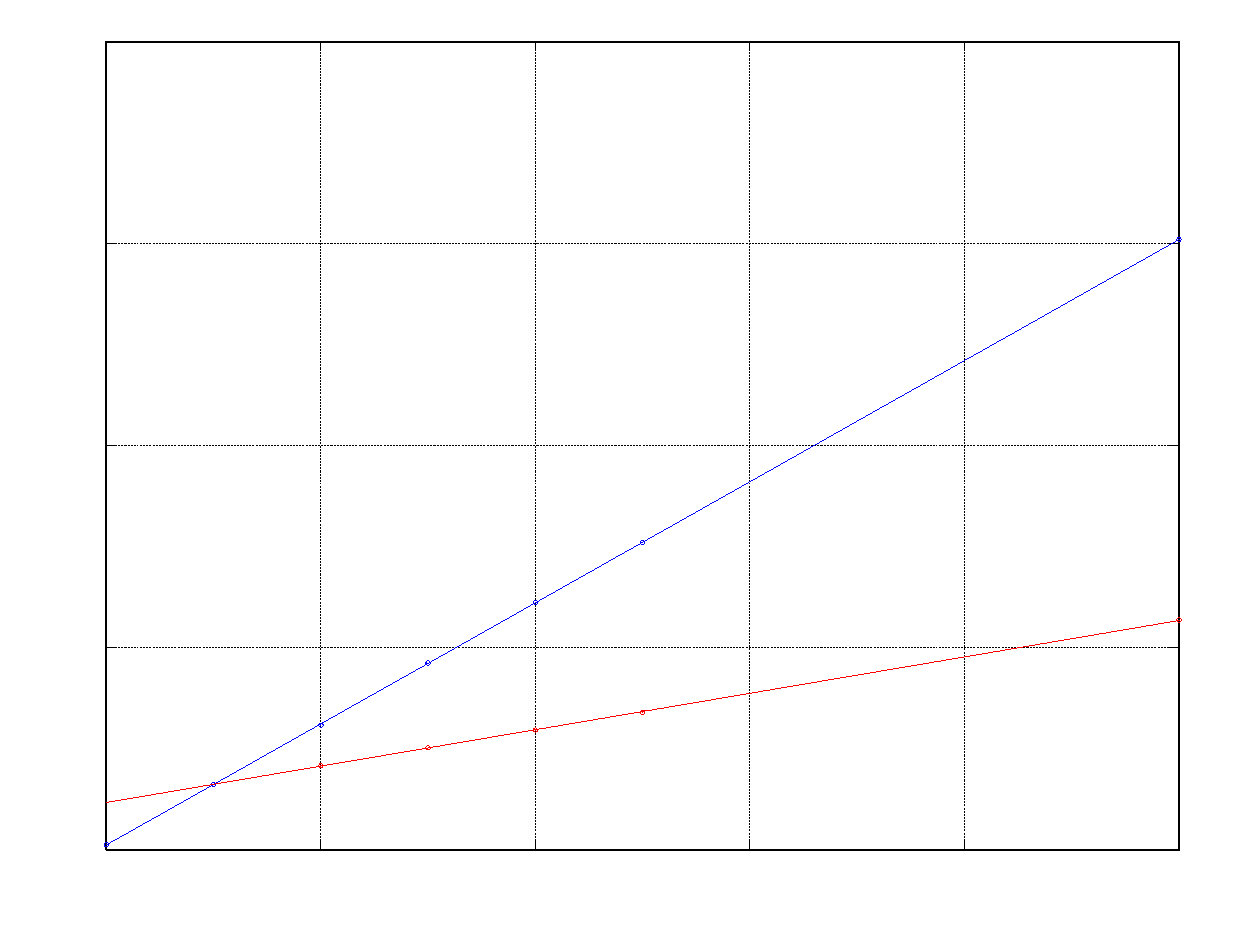
\includegraphics{temps}}%
    \gplfronttext
  \end{picture}%
\endgroup
}
	\caption{Tempo de execução da função de atualização dos temporizadores em função do número de tarefas para 1 temporizador por tarefa e para 1 temporizador global partilhado por todas as tarefas}
	\label{fig:timers}
\end{figure}

\section{Conclusão}

\end{document}
